%!TEX root =conext14.tex
\section{Performance Evaluation}
\label{sec:evaluation}

To evaluate the performance of our proposed system, we implemented our multipath IP in Linux kernel $3.12.1$ under Ubuntu system and install the prototype on two desktops. Both desktops are connected directly to one router without any middle-box. Each desktop has two $100Mbps$ NICs which means that there are totally $4$ paths and the capacity is $200MBps$ between the two nodes. We use Netem\cite{netem} to throttle the connection to evaluate our prototype under multiple scenarios. Wireless connection is also considered in our evaluation.

Besides the controlled lab experiments, we also evaluate MPIP on the Internet to verify NAT immunization and system robustness. We connect our client to a MPIP enabled node in Emulab\cite{emulab} located in Utah . According to our test, the capacity between our client and the server in Emulab is about $5Mbps$, so we limit the bandwidth of both NICs on the client to be $2Mbps$. Because there is only one NIC that connects to Internet on the Emulab node, there are only $2$ paths in this case.

In all experiments, we try to keep the configuration of each node unchanged after installation. We don't do any special configuration to the system, neither we do any optimization to squeeze out all possible throughput. Except specific experiments that can only be applied to MPIP like UDP experiment and customization MPIP routing, we try to do side-by-side comparison with MPTCP for TCP connections. We will figure out how these two features work independently and together as stated in Section~\ref{sec:together};

For all throughput related experiments, we use iperf3 to generate traffic between the client to the server.


\subsection{Clock Offset}
\label{sec:clock}

During our experiments, we found that the clock of each node has some small difference. In our experiment configuration, the clock of the server is slightly faster than the client. Even this error is very small, we still see the difference in a long experiment.
Certainly, nowadays, most computers have NTP enabled and the system's local time synchronize with time server periodically, but we still think that this difference is worth to be shown here.

On our experiment plat, we turn off NTP on both nodes, do a TCP transmission with iperf3 for one day with consistent traffic. Inside MPIP, we record the one-way delay of each packet from the client to server. Because the traffic load is consistent, queuing delay roughly remains the same. But as shown in Figure~\ref{fig.clock}, because of the clock offset between the two nodes, the trend of queuing delay exposes an linearly increasing curve even the trend is very slow. In Figure~\ref{fig.clock}, we record the queuing delay every one minute. For the whole day($1400$ minutes), we can see that the clock offset is about $350$ milliseconds which means that the server's clock runs one millisecond fast than the client for each four minutes. We will be able to see this trend again in following results.

\begin{figure}
\centering{
\subfigure[Clock offset
\label{fig.clock}]{\includegraphics[width=0.49\linewidth,height=1.4in]{fig/clock.eps}}
\subfigure[Out-of-order process
\label{fig.outoforder}]{\includegraphics[width=0.49\linewidth,height=1.4in]{fig/out_of_order_w_sack.eps}}
}
\caption{Clock and Out-of-order}
\label{fig.clockandoutoforder}
\end{figure}


\subsection{TCP Evaluation}
\label{sec:tcp}

As the dominating traffic, TCP plays a critical role in today's Internet. We try to evaluate the performance of MPIP over TCP connections in multiple network configurations. 

\subsubsection{TCP Out-of-order Process}
\label{sec:outoforder}

In Section~\ref{sec:outoforder}, we explained why out-of-order is a problem that must be dealt with in multipath implementations, and we also proposed our solution to this problem. To verify our proposition, we replace one NIC card on the client with a wireless interface. In our experiment plat, the RTT of one path with two wired NICs is about $0.1$ms while paths with one the wireless NIC is about $0.5$ms which will generate enough out-of-order packets. Also, to make sure that there are heavy load of packets to be assigned to the wireless NIC card, instead of using the standard path selection algorithm in Section~\ref{sec:selection}, we fix the weight of all the four paths to be the same. Then we make sure that $50\%$ of outbound packets will be assigned to the wireless NIC.
With this configuration, we do a regular TCP transmission that lasts for $20$ minutes with out-of-order process enabled and disabled respectively. The result is shown in Figure~\ref{fig.outoforder}.

With the same configuration, Figure~\ref{fig.outoforder} shows the improvement brought by the out-of-order process. The average throughput is $XX$Mbps and $XX$Mbps with/out out-of-order process respectively. The improvement maybe trivial if the delay on all the paths is the same because most packets will arrive at the receiver in the order of being sent out. But for multipath connections, it can be very often that each path goes through a totally different route, that is where out-of-order happens most. In all following experiments, we enable out-of-order process by default.

\subsubsection{TCP Throughput Enhancement}
\label{sec:tcptp}

As we mentioned in Section~\ref{sec:tcp}, there are two different implementation of multipath TCP in our system to solve NAT problem which are fake TCP connection and UDP wrapper. We do a specific experiment to evaluate the performance of each approach as shown in Figure~\ref{fig.implementation}. With regular TCP, the average throughput we can achieve is about $92$Mbps. For MPIP, with either fake TCP or UDP wrapper, we both achieve an average throughput of about $165$Mbps. This result shows that both implementations have roughly the same performance. In all following experiments, we use fake TCP by default, but UDP is still kept as an option for users.

\begin{figure}
\centering{
\subfigure[Fake TCP vs UDP Wrapper
\label{fig.implementation}]{\includegraphics[width=0.49\linewidth,height=1.4in]{fig/implementation.eps}}
}
\caption{TCP evaluation}
\label{fig.tcptp}
\end{figure}



\begin{figure*}[htb]
\centering{
\subfigure{\includegraphics[width=0.33\linewidth]{fig/out_of_order_wo_sack.eps}}
\subfigure{\includegraphics[width=0.33\linewidth]{fig/out_of_order_w_sack.eps}}
\subfigure{\includegraphics[width=0.33\linewidth]{fig/clock.eps}}
\subfigure{\includegraphics[width=0.33\linewidth]{fig/implementation.eps}}
\subfigure{\includegraphics[width=0.33\linewidth]{fig/no_limit.eps}}
\subfigure{\includegraphics[width=0.33\linewidth]{fig/no_limit_tp_comp.eps}}
\subfigure{\includegraphics[width=0.33\linewidth]{fig/no_limit_qd_comp.eps}}
\subfigure{\includegraphics[width=0.33\linewidth]{fig/limit.eps}}
\subfigure{\includegraphics[width=0.33\linewidth]{fig/limit_tp_comp.eps}}
\subfigure{\includegraphics[width=0.33\linewidth]{fig/limit_qd_comp.eps}}
\subfigure{\includegraphics[width=0.33\linewidth]{fig/delay_1.eps}}
\subfigure{\includegraphics[width=0.33\linewidth]{fig/delay_tp_comp.eps}}
\subfigure{\includegraphics[width=0.33\linewidth]{fig/delay_qd_com.eps}}
\subfigure{\includegraphics[width=0.33\linewidth]{fig/wireless.eps}}
\subfigure{\includegraphics[width=0.33\linewidth]{fig/wireless_tp_comp.eps}}
}
\caption{Side-by-side comparison for no limit}
\label{fig.no_limit}
\end{figure*}

\begin{figure*}[htb]
\centering{
\subfigure{\includegraphics[width=0.33\linewidth]{fig/wireless_qd_comp.eps}}
\subfigure{\includegraphics[width=0.33\linewidth]{fig/routing_ack.eps}}
\subfigure{\includegraphics[width=0.33\linewidth]{fig/emulab.eps}}
\subfigure{\includegraphics[width=0.33\linewidth]{fig/emulab_tp_comp.eps}}
\subfigure{\includegraphics[width=0.33\linewidth]{fig/emulab_qd_comp.eps}}
\subfigure{\includegraphics[width=0.33\linewidth]{fig/pair_limit.eps}}
\subfigure{\includegraphics[width=0.33\linewidth]{fig/pair_limit_tp_comp.eps}}
\subfigure{\includegraphics[width=0.33\linewidth]{fig/pair_limit_qd_comp.eps}}
\subfigure{\includegraphics[width=0.33\linewidth]{fig/twopath.eps}}
\subfigure{\includegraphics[width=0.33\linewidth]{fig/twopaths_tp_comp.eps}}
\subfigure{\includegraphics[width=0.33\linewidth]{fig/twopaths_qd_comp.eps}}
\subfigure{\includegraphics[width=0.33\linewidth]{fig/skype_tp_comp.eps}}
\subfigure{\includegraphics[width=0.33\linewidth]{fig/skype_delay_comp.eps}}

}
\caption{Side-by-side comparison for no limit}
\label{fig.no_limit}
\end{figure*}


\subsection{Out-of-order evaluation for TCP}
\label{sec:reoder}

To evaluation the effect of out-of-order process in our prototype, we design following experiment. We replace one NIC with wireless NIC, then there will still be $4$ paths. For all the paths, we assign the same path weight which means that every path is assigned the same amount of packets. In this scenario, $50\%$ percent of packets will be sent throughput the wireless NIC. The difference between propagation delay of the wireless path and wired path is large enough to generate a substantial number of out-of-order packets. By enabling and disabling out-of-order functionality, we get Figure~\ref{fig.outoforder}.


\subsection{Skype voice call improvement}
\label{sec:skype}

In Section~\ref{sec:resp}, we mentioned that Skype can benefit from our customized routing for responsiveness. Skype calls has higher requirement on the responsiveness of audio packets. According to our experiments, Skype audio packets are generally less than $200$ bytes. In Table~\ref{tb.route}, for packets that is smaller than $200$ bytes, responsiveness consideration will be the first priority. 

To show how this rule influence Skype audio streaming, we change the delay of NIC cards using the netem package in Ubuntu. On one side of the Skype call, we have two NIC cards as stated above. We ran the experiment for $360$ seconds with $3$ stages. In the first $120$ seconds, there is no manually added delay on each NIC card, we add additional $120ms$ delay to the first NIC card in the following $120$ seconds, finally for the last $120$ seconds, we add $120ms$ delay to the second NIC card. We did our Skype audio experiment without video content while most packets on the connection are audio packets except some control packets. Figure~\ref{fig.skype} shows the packets routing adaptation as the delay value changes. By this adaptation, we can make sure that the audio streaming will always choose the path that has lower delay to keep the best user experience even other paths have the same throughput.


\subsection{Smooth connection switch}
\label{sec:switch}

In Figure~\ref{fig.switch}, we verify that smooth switch between different NIC cards works perfectly over our MPIP implementation by doing an IPERF TCP experiment. We do a side-by-side comparison between MPIP and MPTCP. We also divide the experiment into $3$ sections with $120$ seconds for each section. On the client side of the connection, there are two NIC cards. In the first $120$ seconds, both NIC cards work synchronously, then we disable one of them for $120$ seconds, and during the last $120$ seconds, we enable back the NIC card. The result shows that our MPIP system can follow this on/off process perfectly with stable throughput. For MPTCP, as shown in previous experiments, MPTCP has higher fluctuation than MPIP even MPTCP can achieve higher throughput than MPIP. This happens because in MPTCP, there are more than one TCP connections ($4$ in this experiment), and each connection has its own congestion window. Although congestion control in MPTCP is coupled among different connections, fluctuation have more chances to happen with $4$ relatively independent congestion windows. But in MPIP, one one TCP connection is constructed for each session which means that there is only one congestion windows. In this case, the throughput is more consistent than that of MPTCP.